% Weekly research report — 2026-08-19 — part-based RePaint colour inpainting (s7).
% Build: make figures (once, pulls HF artifacts) && make.
% Every number in the prose is a macro from generated/numbers.tex (derived from the run
% artifacts on HF) — nothing below is hand-typed data.
\documentclass[11pt]{article}
\usepackage{weeklyreport}
% AUTO-GENERATED by make_figures.py from runs/repaint/eval_rows_{auto,labeled_s3}.csv on HF.
% Every number quoted in the report's prose lives here. Do not edit by hand.
%
% Naming: \dE<Stage><Variant><Crop>  mean-of-seeds Delta-E
%         \bok<Stage><Variant><Crop>  best-of-k (min over seeds)
%         \dv<Stage><Variant><Crop>   sample diversity (mean pairwise Delta-E)
%         \eII<Stage><Variant>        E2 (one part fully occluded), 50% crop
%   Stage    : S = synthetic palette, R = real texture
%   Variant  : NN, PM (part-mean), RV (vanilla), RP (part), RO (part, oracle seg), OC (ceiling)
%   Crop     : Lo = 25%, Mid = 50%, Hi = 75%

\newcommand*\dESNNLo{32.9}
\newcommand*\bokSNNLo{32.9}
\newcommand*\dESNNMid{49.1}
\newcommand*\bokSNNMid{49.1}
\newcommand*\dESNNHi{60.8}
\newcommand*\bokSNNHi{60.8}
\newcommand*\eIISNN{65.8}
\newcommand*\dESPMLo{32.8}
\newcommand*\bokSPMLo{32.8}
\newcommand*\dESPMMid{38.7}
\newcommand*\bokSPMMid{38.7}
\newcommand*\dESPMHi{51.1}
\newcommand*\bokSPMHi{51.1}
\newcommand*\eIISPM{57.5}
\newcommand*\dESRVLo{32.4}
\newcommand*\bokSRVLo{29.7}
\newcommand*\dvSRVLo{18.1}
\newcommand*\dESRVMid{39.8}
\newcommand*\bokSRVMid{37.3}
\newcommand*\dvSRVMid{18.2}
\newcommand*\dESRVHi{34.5}
\newcommand*\bokSRVHi{32.7}
\newcommand*\dvSRVHi{18.2}
\newcommand*\eIISRV{11.2}
\newcommand*\dESRPLo{22.6}
\newcommand*\bokSRPLo{22.5}
\newcommand*\dvSRPLo{9.7}
\newcommand*\dESRPMid{23.5}
\newcommand*\bokSRPMid{23.4}
\newcommand*\dvSRPMid{9.2}
\newcommand*\dESRPHi{22.5}
\newcommand*\bokSRPHi{22.5}
\newcommand*\dvSRPHi{8.4}
\newcommand*\eIISRP{16.8}
\newcommand*\dESROLo{16.1}
\newcommand*\bokSROLo{16.0}
\newcommand*\dvSROLo{9.6}
\newcommand*\dESROMid{17.6}
\newcommand*\bokSROMid{17.5}
\newcommand*\dvSROMid{9.2}
\newcommand*\dESROHi{15.8}
\newcommand*\bokSROHi{15.7}
\newcommand*\dvSROHi{8.2}
\newcommand*\eIISRO{18.3}
\newcommand*\dESOCLo{5.4}
\newcommand*\bokSOCLo{5.4}
\newcommand*\dESOCMid{5.3}
\newcommand*\bokSOCMid{5.3}
\newcommand*\dESOCHi{5.3}
\newcommand*\bokSOCHi{5.3}
\newcommand*\dERNNLo{19.2}
\newcommand*\bokRNNLo{19.2}
\newcommand*\dERNNMid{22.7}
\newcommand*\bokRNNMid{22.7}
\newcommand*\dERNNHi{24.1}
\newcommand*\bokRNNHi{24.1}
\newcommand*\eIIRNN{25.3}
\newcommand*\dERPMLo{20.2}
\newcommand*\bokRPMLo{20.2}
\newcommand*\dERPMMid{24.5}
\newcommand*\bokRPMMid{24.5}
\newcommand*\dERPMHi{27.1}
\newcommand*\bokRPMHi{27.1}
\newcommand*\eIIRPM{17.8}
\newcommand*\dERRVLo{54.5}
\newcommand*\bokRRVLo{48.7}
\newcommand*\dvRRVLo{46.7}
\newcommand*\dERRVMid{62.2}
\newcommand*\bokRRVMid{55.6}
\newcommand*\dvRRVMid{50.5}
\newcommand*\dERRVHi{68.6}
\newcommand*\bokRRVHi{63.2}
\newcommand*\dvRRVHi{53.5}
\newcommand*\eIIRRV{65.4}
\newcommand*\dERRPLo{45.4}
\newcommand*\bokRRPLo{41.0}
\newcommand*\dvRRPLo{26.5}
\newcommand*\dERRPMid{61.0}
\newcommand*\bokRRPMid{52.8}
\newcommand*\dvRRPMid{31.4}
\newcommand*\dERRPHi{79.4}
\newcommand*\bokRRPHi{75.2}
\newcommand*\dvRRPHi{25.4}
\newcommand*\eIIRRP{84.6}
\newcommand*\dERROLo{44.4}
\newcommand*\bokRROLo{39.6}
\newcommand*\dvRROLo{27.5}
\newcommand*\dERROMid{61.1}
\newcommand*\bokRROMid{52.7}
\newcommand*\dvRROMid{32.3}
\newcommand*\dERROHi{77.4}
\newcommand*\bokRROHi{72.6}
\newcommand*\dvRROHi{25.6}
\newcommand*\eIIRRO{86.4}
\newcommand*\dEROCLo{18.7}
\newcommand*\bokROCLo{18.7}
\newcommand*\dEROCMid{18.7}
\newcommand*\bokROCMid{18.7}
\newcommand*\dEROCHi{18.9}
\newcommand*\bokROCHi{18.9}
\newcommand*\winS{99}
\newcommand*\winNS{110}
\newcommand*\winES{96}
\newcommand*\winENS{109}
\newcommand*\hdrmS{33.4}
\newcommand*\nrowsS{6{,}809}
\newcommand*\nmodS{110}
\newcommand*\bestbaseS{part-mean}
\newcommand*\winR{0}
\newcommand*\winNR{34}
\newcommand*\winER{0}
\newcommand*\winENR{34}
\newcommand*\hdrmR{4.0}
\newcommand*\nrowsR{2{,}108}
\newcommand*\nmodR{34}
\newcommand*\bestbaseR{NN-copy}
\newcommand*\ratioS{0.61}
\newcommand*\ratioR{2.69}
\newcommand*\nLabeled{137}
\newcommand*\datasetRev{2fa9f9b821}
\newcommand*\hdrmRatio{8.4}
\newcommand*\dvRatio{3.4}
\newcommand*\sixLearned{0.0727}
\newcommand*\sixMean{0.0696}
\newcommand*\sixRatio{1.045}


\reporttitle{Can a learned colour prior beat a trivial one?\\Part-based RePaint on completed point clouds}
\reportweek{2026-08-19}
\reportdates{7--19 August 2026}
\reportauthors{Efe Yenice (researcher) \textperiodcentered\ Claude (AI co-researcher)\\[2pt]
\small method and original notebooks: \textbf{Pelin K\i l\i\c{c}} \textperiodcentered\ port, scaling, controls and evaluation: this project}
\reportquestion{when the geometry is already complete, can a diffusion colour prior colour the missing points better than copying or averaging the visible ones?}
\reportrepo{\texttt{efeyenice/point-cloud-completion-research} \textperiodcentered\ \texttt{reports/2026-08-19-repaint-color}}

\begin{document}
\reportheader

\begin{tldr}
\begin{enumerate}
  \item \textbf{On real texture the method loses decisively --- and we can say exactly why.}
  The diffusion colour prior scores \dERRPMid{} $\Delta$E against \dERNNMid{} for NN-copy and
  \dERPMMid{} for part-mean, winning \winR{} of \winNR{} test models. Four independent controls
  rule out the mundane explanations (\cref{sec:trust}).
  \item \textbf{The reason is structural, not a bug: the prize collapsed.} On real texture the
  \emph{oracle ceiling} --- part-mean given perfect labels, the best \emph{any} part-colour
  method could achieve --- is \dEROCMid, while the best trivial rule already scores
  \dERNNMid. The entire margin available to this whole class of methods is
  \textbf{\hdrmR\,$\Delta$E} ($\approx$2 just-noticeable differences), against \hdrmS\,$\Delta$E
  on synthetic colours: a \hdrmRatio$\times$ collapse (\cref{fig:headroom}). The method was not
  merely beaten; it was playing for almost nothing.
  \item \textbf{The same code wins on synthetic colours, which is what makes the negative
  readable.} At \dESRPMid{} vs.\ \dESPMMid/\dESNNMid{} it wins \winS/\winNS{} models and stays
  flat as occlusion grows while the copy rules decay --- textbook ``a prior helps when
  evidence disappears''. On real texture that behaviour inverts exactly
  (\cref{fig:scissors}). Prior \emph{learnability}, not implementation, is the variable.
\end{enumerate}
\end{tldr}

\section{The story so far: why we reached for a generative model}\label{sec:story}

The project asks whether per-point colour helps completion, and under what conditions. Two
previous results set up this week. First, the s5 arms: a learned colour head that predicted
RGB for the completed cloud never beat \emph{mean-copy} --- the trivial rule ``paint every
missing point the average colour of the visible ones''. Second, the s6 data-scale curve: at
$N{=}150$ models/category the learned head reached \sixLearned{} colour MSE against
mean-copy's \sixMean. More data narrowed nothing that mattered.

Both are symptoms of one mechanism. Completion is \emph{ambiguous}: the occluded region is
unobserved, so many colourings are consistent with the same visible evidence. A regressor
trained under a squared-error loss is rewarded for predicting the \emph{conditional mean} of
that set of possibilities --- so when it cannot tell red from blue, the loss actively pushes
it toward washed-out grey. Mean-copy is not a weak opponent to be out-engineered; under an
L2-type metric it is close to what the optimal \emph{point} predictor does. You cannot train
your way past it with a bigger regressor.

The principled escape is to stop asking for one error-minimising answer and instead learn a
\emph{distribution} over plausible answers, then draw one committed sample from it. That is
the generative turn (ADR-0009), and this week is its first concrete instrument: a colour
prior, adopted from our collaborator's line of work (ADR-0010), tested honestly at scale.

\section{The method}\label{sec:method}

Geometry is not the problem here --- a frozen, pretrained PoinTr already completes the shape,
and we do not touch it. The open question is how the \emph{filled-in points get coloured}.

\begin{center}
\begin{tikzpicture}[
  node distance=5mm and 6mm,
  box/.style={draw=wrnavy, rounded corners=1.5pt, fill=wrnavy!5, font=\scriptsize,
              align=center, inner sep=3pt, minimum height=9mm, text width=19mm},
  model/.style={box, fill=wraccent!14},
  arr/.style={-{Stealth[length=2mm]}, thick, color=wrnavy}]
  \node[box]              (part)  {partial scan\\xyz + rgb};
  \node[model, right=of part] (pointr) {\textbf{frozen PoinTr}\\geometry only};
  \node[box, right=of pointr] (union) {union cloud\\known + unknown};
  \node[model, right=of union] (seg) {PointNet\\part labels};
  \node[model, right=of seg]  (rep) {\textbf{colour DDPM}\\+ RePaint};
  \node[box, right=of rep]   (score) {$\Delta$E on the\\missing region};
  \draw[arr] (part) -- (pointr);
  \draw[arr] (pointr) -- (union);
  \draw[arr] (union) -- (seg);
  \draw[arr] (seg) -- (rep);
  \draw[arr] (rep) -- (score);
  \draw[arr] (part.south) to[bend right=22] node[font=\tiny\itshape, below, color=wrgray]
    {visible colours (known)} (union.south);
\end{tikzpicture}
\end{center}

The central object is the \textbf{union cloud}: the visible partial points, whose colours we
\emph{know}, glued to PoinTr's filled-in points, whose colours must be \emph{invented}. Only
the invented region is ever scored.

\begin{primer}{Background: diffusion, and how RePaint conditions it without retraining}
A \textbf{DDPM} learns by destroying and rebuilding. Take real data, add a little Gaussian
noise repeatedly ($T{=}200$ steps here) until nothing but noise remains; train a network to
undo \emph{one} step. To generate, start from pure noise and run those steps backwards. Here
the diffused signal is \textbf{not geometry} --- it is the per-point RGB field sitting on
fixed, already-completed coordinates. The model learns ``what do plausible aeroplane
colourings look like?''

\textbf{RePaint} (Lugmayr et al., CVPR 2022) makes that unconditional model do inpainting
\emph{without ever training it on masks}. At each reverse step the known points are
overwritten with the true colours, noised to that step's level; the unknown points keep the
model's guess. Every so often the sampler jumps \emph{back up} in noise and re-denoises
(``time travel''), letting the invented region re-negotiate with the known one so the result
agrees semantically, not just at the seam. One trained model then serves every occlusion
ratio with no retraining --- which is exactly why the occlusion sweep below is cheap.
\end{primer}

\begin{center}
\begin{tikzpicture}[
  every node/.style={font=\scriptsize},
  st/.style={draw=wrnavy, circle, fill=wrnavy!6, inner sep=1.6pt, minimum size=8mm},
  arr/.style={-{Stealth[length=1.8mm]}, thick, color=wrnavy},
  kn/.style={draw=wraccent, rounded corners=1.5pt, fill=wraccent!12, inner sep=3pt, align=center}]
  \node[st] (xT)  {$x_T$};
  \node[st, right=9mm of xT]  (xt)  {$x_t$};
  \node[st, right=9mm of xt]  (xa)  {$x_{t-1}$};
  \node[st, right=9mm of xa]  (xb)  {$x_{t-2}$};
  \node[st, right=9mm of xb]  (x0)  {$x_0$};
  \draw[arr, dotted] (xT) -- (xt);
  \draw[arr] (xt) -- node[above, font=\tiny] {denoise} (xa);
  \draw[arr] (xa) -- node[above, font=\tiny] {denoise} (xb);
  \draw[arr, dotted] (xb) -- (x0);
  \node[kn, above=7mm of xa] (known) {\textbf{known colours} (visible points),\\noised to the current step};
  \foreach \n in {xt,xa,xb}{\draw[arr, color=wraccent, densely dashed] (known) -- (\n);}
  \draw[arr, color=wrgray] (xb.south) to[bend left=38]
    node[below, font=\tiny\itshape, color=wrgray] {time-travel jump: re-noise and denoise again} (xa.south);
  \node[right=3mm of x0, font=\tiny\itshape, color=wrgray, text width=22mm]
    {final colours for the missing points};
\end{tikzpicture}
\end{center}

\textbf{``Part-based''} is our collaborator's addition, in three places: the denoiser pools
features \emph{within each part} (a learned analogue of the part-mean rule, making cross-part
colour bleed structurally hard); a part with \emph{zero} visible points is flagged
\emph{anchorless} and filled from the prior rather than from a neighbouring part's colour;
and the resampling budget grows with the worst part's occlusion.

\section{The experiment}\label{sec:exp}

\subsection{Two stages, run as one controlled comparison}

The same code, metric and protocol are run over two colour regimes, so that
\emph{prior-learnability} is the manipulated variable:

\begin{itemize}
  \item \textbf{Synthetic palette} --- each part is one flat colour plus a little noise
  (\nmodS{} test models, \nrowsS{} measurements). \emph{Honest caveat, stated up front:} where
  every part is a single flat colour, part-mean with good labels is close to Bayes-optimal and
  intra-part texture gains cannot appear. This stage validates \emph{the machine}, not the
  texture claim.
  \item \textbf{Real texture} --- colours sampled from textured ShapeNet meshes
  (\nmodR{} test models, \nrowsR{} measurements). \textbf{This is the experiment.} The labelled
  data was built by us: \nLabeled{} aeroplanes fused from our own HF bundles with
  ShapeNet-Part labels, frame-QA'd, refusing any model whose label transfer stays poor rather
  than writing bad labels.
\end{itemize}

\subsection{Six rows, because a single number cannot be diagnosed}

Every cell of every table reports the same metric --- \textbf{mean $\Delta$E(Lab) over the
missing region only}, on unseen test models. $\Delta$E is perceptual colour distance;
$\approx$2 is the threshold of visibility. Six rows are computed so that a result can be
\emph{explained}, not merely reported:

\begin{center}\footnotesize
\begin{tabular}{lll}
\toprule
row & what it predicts & what it isolates \\
\midrule
NN-copy      & nearest visible point's colour        & trivial local copying \\
part-mean    & mean visible colour of that part      & the strongest trivial rule \\
oracle ceiling & part-mean, \emph{ground-truth} labels & the best \emph{any} part-colour method can do \\
RePaint-vanilla & the DDPM, no part conditioning & whether ``part-based'' earns its keep \\
RePaint-part & \textbf{the method under test}        & --- \\
RePaint-part (oracle seg) & the method, ground-truth labels & segmentation error \\
\bottomrule
\end{tabular}
\end{center}

Two further axes: \textbf{E1} sweeps occlusion over $\{25, 50, 75\}\%$ --- promised in the
original notebooks but never run --- and \textbf{E2} removes one part entirely (the
\emph{anchorless} case the method was designed for; the part is dropped by \emph{ground-truth}
label, because dropping by the segmenter silently degenerates when the segmenter never
predicts that part). Because a sampler is structurally penalised by single-sample scoring,
each diffusion row is drawn five times per model and reported as \textbf{mean-of-seeds}
(the honest row), \textbf{best-of-$k$} (does the prior \emph{cover} the truth?) and
\textbf{diversity} (mean pairwise $\Delta$E between samples).

\section{Results}\label{sec:results}

\begin{figure}[t]
  \centering
  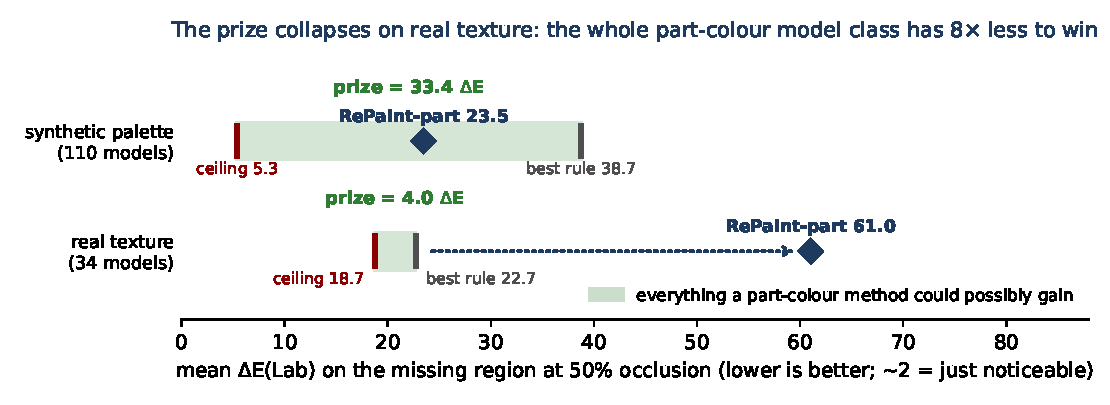
\includegraphics[width=\textwidth]{figures/fig_headroom.pdf}
  \caption{\textbf{The prize collapses.} The shaded band is everything a part-colour method
  could possibly gain: from the best trivial rule down to the oracle ceiling. On synthetic
  colours it spans \hdrmS\,$\Delta$E and RePaint-part lands inside it. On real texture it is
  only \hdrmR\,$\Delta$E wide --- about two just-noticeable differences --- and the method
  lands far outside it.}
  \label{fig:headroom}
\end{figure}

\subsection{The headline: a collapsed margin, and a method outside it}\label{sec:headline}

\Cref{fig:headroom} is the week's finding. On real texture the oracle ceiling sits at
\dEROCMid{} while NN-copy already achieves \dERNNMid: perfect part labels plus a perfect
per-part average buy only \hdrmR\,$\Delta$E over naive copying. Real aeroplane texture is
simply not well described by one colour per part --- the residual is intra-part variation that
no part-level model can represent. On synthetic colours the same measurement gives
\hdrmS\,$\Delta$E of room, a \hdrmRatio$\times$ difference.

That single fact reframes the result. RePaint-part scoring \dERRPMid{} against \dERNNMid{} is
not a near miss inside a rich design space; it is a method competing for a margin that had
already almost vanished, and overshooting it by an order of magnitude.

\begin{table}[h]
  \centering\small
  \begin{tabular}{lrrrr}
    \toprule
    & \multicolumn{2}{c}{synthetic palette} & \multicolumn{2}{c}{real texture} \\
    \cmidrule(lr){2-3}\cmidrule(lr){4-5}
    variant & mean & best-of-$k$ & mean & best-of-$k$ \\
    \midrule
    NN-copy                   & \dESNNMid & \bokSNNMid & \textbf{\dERNNMid} & \bokRNNMid \\
    part-mean                 & \dESPMMid & \bokSPMMid & \dERPMMid & \bokRPMMid \\
    oracle ceiling            & \dESOCMid & \bokSOCMid & \dEROCMid & \bokROCMid \\
    \midrule
    RePaint-vanilla           & \dESRVMid & \bokSRVMid & \dERRVMid & \bokRRVMid \\
    RePaint-part              & \textbf{\dESRPMid} & \bokSRPMid & \dERRPMid & \bokRRPMid \\
    RePaint-part (oracle seg) & \dESROMid & \bokSROMid & \dERROMid & \bokRROMid \\
    \bottomrule
  \end{tabular}
  \caption{Mean $\Delta$E(Lab) on the missing region at 50\,\% occlusion (lower is better);
  best-of-$k$ is the minimum over 5 seeds per model. Models won by RePaint-part against the
  better trivial rule: \winS/\winNS{} synthetic, \winR/\winNR{} real. Full sweep in
  \cref{app:sweep}.}
  \label{tab:headline}
\end{table}

\subsection{Occlusion: the behaviour inverts}\label{sec:sweep}

\begin{figure}[h]
  \centering
  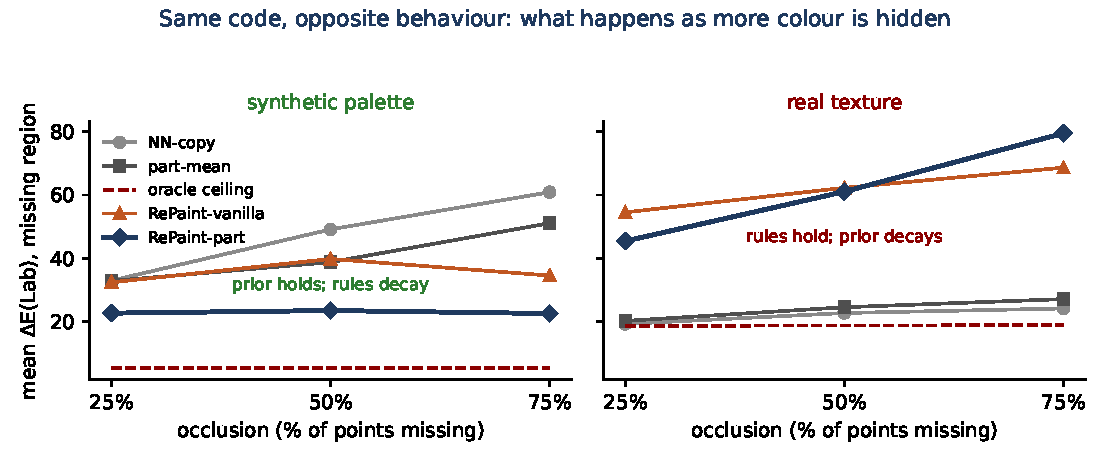
\includegraphics[width=\textwidth]{figures/fig_scissors.pdf}
  \caption{\textbf{The occlusion sweep.} As more colour is hidden, a genuine prior should
  matter \emph{more} and copy rules should decay. That is exactly the synthetic picture
  (RePaint-part flat at \dESRPLo$\rightarrow$\dESRPHi{} while NN-copy climbs
  \dESNNLo$\rightarrow$\dESNNHi). On real texture it inverts: the rules stay flat and the
  prior degrades \dERRPLo$\rightarrow$\dERRPHi.}
  \label{fig:scissors}
\end{figure}

This sweep is the most diagnostic axis we added, and it separates the two stages cleanly. When
the prior is learnable, hiding more colour hurts the copy rules (less to copy from) and barely
touches the prior --- the classic argument for generative completion. When the prior is
\emph{not} learnable, hiding more colour simply hands more of the output over to a bad prior,
so the method degrades while the rules, which still have local evidence, hold.

The anchorless case (\textbf{E2}, one part entirely missing) makes the same point at its
extreme. It is the scenario the method exists for, and on synthetic colours it delivers
crushingly: \eIISRP{} against \eIISPM{} for part-mean. On real texture it fails hardest of
all: \eIIRRP{} against \eIIRPM.

\subsection{What it looks like}\label{sec:qual}

\begin{figure}[t]
  \centering
  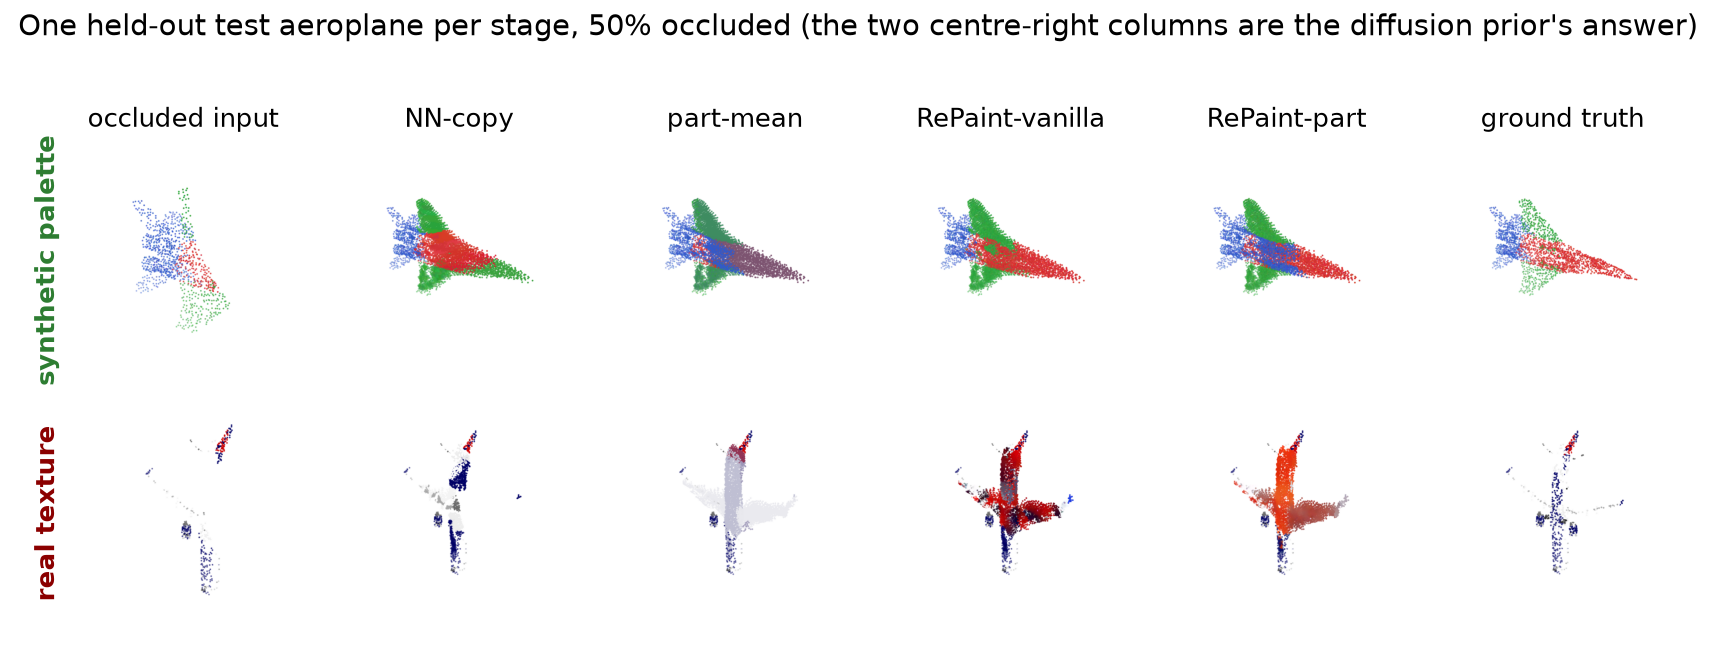
\includegraphics[width=\textwidth]{figures/fig_panels.png}
  \caption{\textbf{The mechanism, visible.} Top row (synthetic): the prior reconstructs the
  part colours convincingly. Bottom row (real texture): the ground-truth aeroplane is
  predominantly white, and the prior confidently paints a red-orange livery over it. This is
  not blur or hedging --- it is a committed, plausible, wrong answer, which is precisely what
  sampling from an under-trained prior produces.}
  \label{fig:panels}
\end{figure}

\Cref{fig:panels} shows why the failure is interesting rather than embarrassing. The regression
failures of s5/s6 looked like \emph{washed-out} colour --- hedging toward the mean. This
failure looks the opposite: vivid and confident, and wrong. The model has learned that
aeroplanes have liveries; it has not learned which livery \emph{this} aeroplane has, because
roughly a hundred training clouds cannot teach that. Sampling replaced the hedging with
commitment, exactly as intended --- and commitment without knowledge is worse than hedging.

\begin{figure}[h]
  \centering
  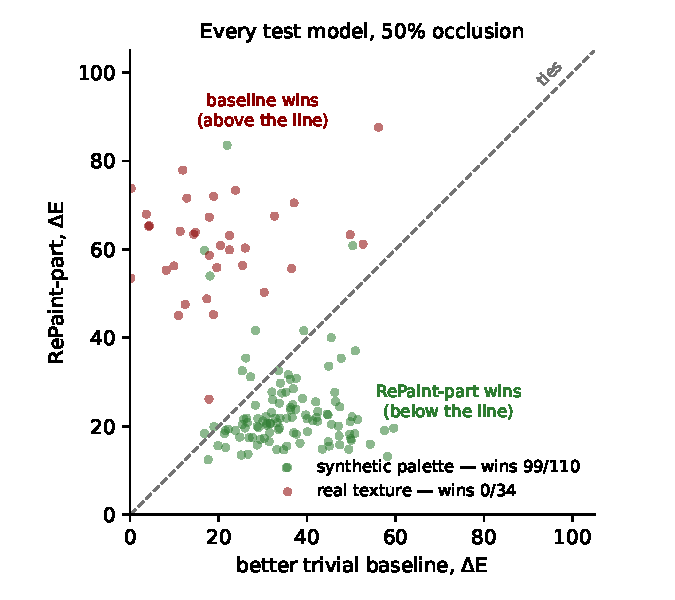
\includegraphics[width=0.62\textwidth]{figures/fig_winloss.pdf}
  \caption{\textbf{Every test model.} Points below the diagonal are models where RePaint-part
  beat the better trivial rule. The two stages separate almost completely; the real-texture
  loss is not an average dragged down by a few outliers.}
  \label{fig:winloss}
\end{figure}

\section{Why we trust the negative}\label{sec:trust}

\begin{figure}[h]
  \centering
  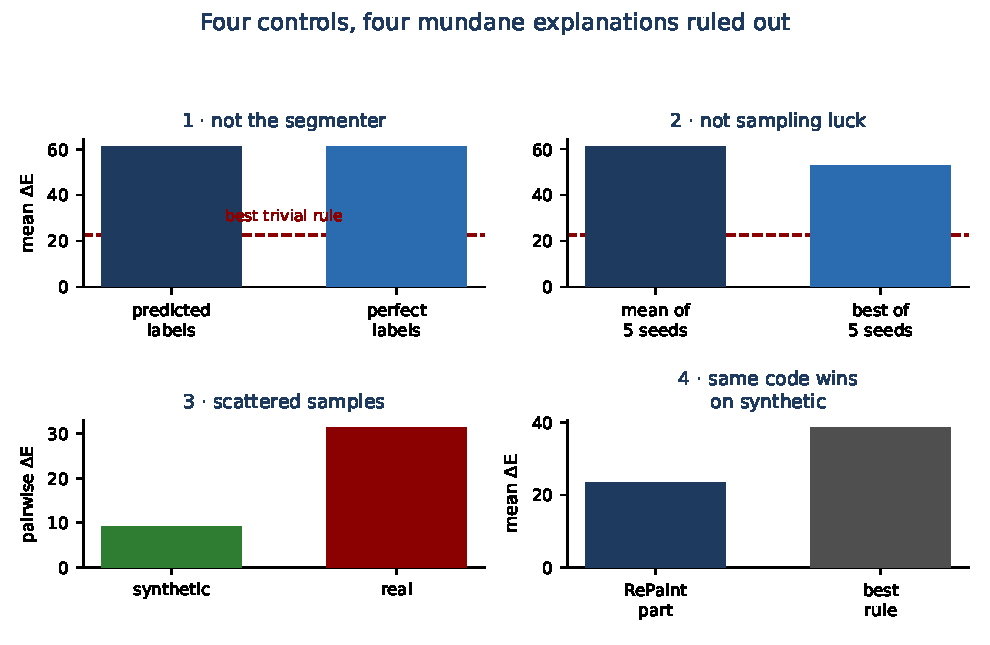
\includegraphics[width=\textwidth]{figures/fig_controls.pdf}
  \caption{\textbf{Four controls.} Each rules out one ordinary explanation for the loss.}
  \label{fig:controls}
\end{figure}

A negative result is only worth reporting if the boring explanations are excluded. Four
controls, each built into the protocol in advance, do that:

\begin{enumerate}
  \item \textbf{Not the segmenter.} Given \emph{ground-truth} part labels the method scores
  \dERROMid{} --- statistically indistinguishable from \dERRPMid{} with predicted labels.
  This matters because it is precisely the confound that made the collaborator's first pass
  inconclusive (a segmenter that never predicted one of the parts); removing it leaves the
  result unchanged.
  \item \textbf{Not sampling luck.} Taking the \emph{best} of five independent draws per model
  still gives \bokRRPMid, more than twice the best trivial rule. The prior does not merely
  miss on average --- it does not cover the right answer at all.
  \item \textbf{Not a near miss.} Sample diversity is \dvRRPMid\,$\Delta$E on real texture
  against \dvSRPMid{} on synthetic. Since $\approx$2 is just-noticeable, the real-texture
  samples are scattered across wildly different colour schemes: an uncommitted prior, not a
  tight distribution centred slightly off-target.
  \item \textbf{Not the code.} The identical pipeline wins \winS/\winNS{} models on synthetic
  colours. Training, sampling, conditioning and metric all work.
\end{enumerate}

The mechanism that survives is the simple one: \textbf{an unconditional colour prior trained on
of the order of a hundred real-texture clouds is too weak, and sampling-time conditioning
cannot extract structure the prior never learned.} RePaint can re-inject known colours and
harmonise around them; it cannot invent knowledge of \emph{this} object's colour scheme.

\section{What the scaling bought us}\label{sec:new}

Running this as a formal experiment rather than a demonstration produced three findings that a
4-model, single-seed pass could not have shown.

\begin{figure}[h]
  \centering
  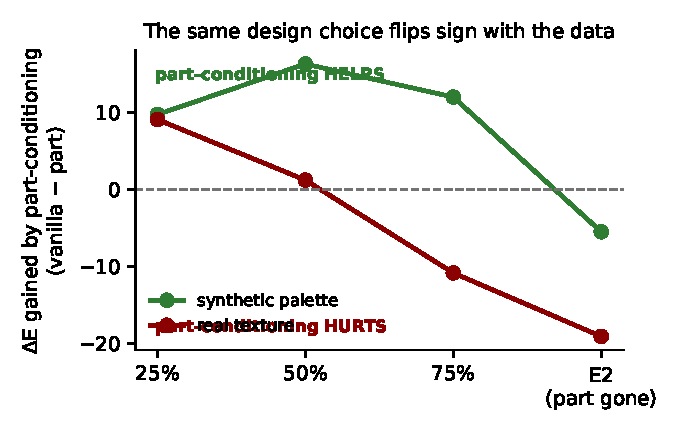
\includegraphics[width=0.60\textwidth]{figures/fig_signflip.pdf}
  \caption{\textbf{Part-conditioning is not universally good.} Its advantage shrinks as
  occlusion grows in \emph{both} regimes, and on real texture it crosses into active harm.}
  \label{fig:signflip}
\end{figure}

\begin{itemize}
  \item \textbf{The headroom collapse} (\cref{sec:headline}) --- the structural result, and the
  one that generalises beyond this method: on real ShapeNet texture, \emph{any} model that
  assigns one colour per part is confined to a \hdrmR\,$\Delta$E margin.
  \item \textbf{Part-conditioning flips sign} (\cref{fig:signflip}). On synthetic colours it
  helps substantially at every occlusion level of E1 (\dESRPMid{} vs.\ \dESRVMid{} at
  50\,\%), but its benefit decays as occlusion grows, and in the anchorless case it is already
  \emph{negative} (\eIISRP{} vs.\ \eIISRV). On real texture the reversal comes earlier and
  harder: helpful at 25\,\%, neutral at 50\,\%, clearly harmful by 75\,\%
  (\dERRPHi{} vs.\ \dERRVHi) and worst at E2 (\eIIRRP{} vs.\ \eIIRRV). The reading is that
  part-pooling makes the model \emph{commit harder} to a part-level colour decision --- which
  is a gain when the part colour is learnable and a penalty when it is not.
  \item \textbf{Diversity is measurable, and it is the tell.} The $\approx$\dvRatio$\times$
  difference in sample spread between regimes (\dvSRPMid{} vs.\ \dvRRPMid) is the most direct
  read-out of prior quality we have, and it comes free from the same samples.
\end{itemize}

\section{Honest read}\label{sec:read}

\begin{itemize}
  \item \textbf{What we can claim.} Within one category (aeroplanes), at this data scale, on
  real texture, part-based RePaint colour inpainting does not beat trivial local colour rules,
  and the failure is attributable to prior weakness rather than to segmentation, sampling
  variance, or implementation. Independently: the part-colour model class itself has
  \hdrmR\,$\Delta$E of headroom on this data.
  \item \textbf{What we cannot claim.} That the method is bad in general. It is untested at
  larger data scales, on other categories, and with trained (rather than sampling-time)
  conditioning. Our real-texture set is \nLabeled{} models of one category; the prior is
  trained on roughly a hundred of them. Nothing here says the approach fails with $10\times$
  the data --- only that it fails with this much.
  \item \textbf{What the synthetic stage does and does not prove.} It proves the machine is
  correct and that RePaint's occlusion behaviour is real. It cannot prove a texture claim,
  because part-mean is near-optimal there by construction.
  \item \textbf{On the collaborator's earlier numbers.} Her real-texture first pass
  (4 models, 1 seed, with a part-segmenter that never predicted one of the parts) was
  explicitly not presented as a result, and this work does not contradict it --- it supplies
  the verdict that setup could not.
\end{itemize}

\begin{table}[h]
  \centering\small
  \begin{tabular}{llll}
    \toprule
    phase & what predicted colour & its trivial baseline & beat it? \\
    \midrule
    s5 & decoupled learned colour head & mean-copy & no \\
    s6 & the same head, $N{=}150$/cat  & mean-copy (\sixMean{} vs.\ \sixLearned) & no ($\times$\sixRatio) \\
    s7 & RePaint diffusion colour prior & NN-copy (\dERNNMid{} vs.\ \dERRPMid) & no ($\times$\ratioR) \\
    \bottomrule
  \end{tabular}
  \caption{\textbf{The through-line.} Three different mechanisms --- a regression head, the
  same head with more data, and a generative prior --- have now failed to beat trivial local
  colour statistics on real texture. \emph{Caveat:} s6 is RGB-MSE and s7 is $\Delta$E(Lab),
  measured in different pipelines; the ratios are within-phase and dimensionless, and the
  pattern is qualitative. Cross-pipeline magnitudes are not comparable (ADR-0007). s5's
  magnitude is superseded and is quoted only as an outcome.}
  \label{tab:throughline}
\end{table}

\Cref{tab:throughline} is the most useful thing to carry forward. The consistent obstacle is
not any one architecture; it is that per-point colour on real ShapeNet texture appears to be
dominated by object-specific information that is not learnable, as a transferable rule, at the
scales we can currently reach. Two of the three attempts failed by hedging; the third failed by
committing. That is a statement about the data, and it is worth more than another architecture
would have been.

\section{Proposed next steps}\label{sec:next}

\begin{enumerate}
  \item \textbf{More textured training data --- the top lever.} Everything above points here.
  \nLabeled{} aeroplanes support a prior trained on $\sim$100 clouds; 107 chairs and 51 cars
  are already label-capable through the same fusion path, and the background data generator can
  extend the bundles. This is the one change the diagnosis directly recommends.
  \item \textbf{Trained conditioning instead of sampling-time only.} Show the mask during
  training. This is also the bridge to ADR-0009's geometry-diffusion spine, and it gives a
  second conditioning mechanism to compare against RePaint on identical data.
  \item \textbf{Condition on a per-object colour scheme.} The panel failure is a model that
  knows aeroplanes have liveries but not which one; a global colour code would remove exactly
  that ambiguity, and it is cheap to test.
  \item \textbf{Escape the part-colour class.} Given a \hdrmR\,$\Delta$E ceiling, any further
  work confined to one-colour-per-part is capped. Intra-part texture modelling is where the
  remaining error actually lives.
  \item \textbf{Deprioritised: segmentation repair}, capacity and $T$ tuning --- the oracle-seg
  control already shows these are not the binding constraint.
\end{enumerate}

\begin{processbox}
\textbf{Roles.} Method and original notebooks: Pelin K\i l\i\c{c}. Efe: direction, decisions at
forks, and the Colab runs. Claude (AI co-researcher): the production port and its tests, the
fused labelled dataset, experiment and control design, analysis, and this report.
\textbf{The loop} (\texttt{docs/WORKFLOW.md}): decide $\rightarrow$ grill the plan $\rightarrow$
ADR $\rightarrow$ build + test locally $\rightarrow$ run resiliently on Colab $\rightarrow$
analyse $\rightarrow$ document + report. \textbf{This fortnight in numbers:} 1 ADR (0010),
2 tested modules (18 unit tests, all green before any GPU time), 1 notebook (18 cells, both
stages), \nLabeled{} labelled models fused by us, \nrowsS{} + \nrowsR{} evaluation measurements,
zero lost work across VM recycles. Timeline and incidents: \cref{app:process}.
\end{processbox}

\clearpage
\appendix

\section{Full sweep --- both stages, all occlusion levels}\label{app:sweep}

\begin{center}\footnotesize\setlength{\tabcolsep}{5pt}
% AUTO-GENERATED by make_figures.py — the full E1/E2 sweep, both stages.
\begin{tabular}{llrrrrrr}
\toprule
& & \multicolumn{3}{c}{synthetic palette} & \multicolumn{3}{c}{real texture} \\
\cmidrule(lr){3-5}\cmidrule(lr){6-8}
table & variant & 25\% & 50\% & 75\% & 25\% & 50\% & 75\% \\
\midrule
E1 & NN-copy & 32.9 & 49.1 & 60.8 & 19.2 & 22.7 & 24.1 \\
E1 & part-mean & 32.8 & 38.7 & 51.1 & 20.2 & 24.5 & 27.1 \\
E1 & oracle ceiling & 5.4 & 5.3 & 5.3 & 18.7 & 18.7 & 18.9 \\
E1 & RePaint-vanilla & 32.4 & 39.8 & 34.5 & 54.5 & 62.2 & 68.6 \\
E1 & RePaint-part & 22.6 & 23.5 & 22.5 & 45.4 & 61.0 & 79.4 \\
E1 & RePaint-part (oracle seg) & 16.1 & 17.6 & 15.8 & 44.4 & 61.1 & 77.4 \\
\midrule
E2 & NN-copy & -- & 65.8 & -- & -- & 25.3 & -- \\
E2 & part-mean & -- & 57.5 & -- & -- & 17.8 & -- \\
E2 & RePaint-vanilla & -- & 11.2 & -- & -- & 65.4 & -- \\
E2 & RePaint-part & -- & 16.8 & -- & -- & 84.6 & -- \\
E2 & RePaint-part (oracle seg) & -- & 18.3 & -- & -- & 86.4 & -- \\
\midrule
DIV & RePaint-vanilla & 18.1 & 18.2 & 18.2 & 46.7 & 50.5 & 53.5 \\
DIV & RePaint-part & 9.7 & 9.2 & 8.4 & 26.5 & 31.4 & 25.4 \\
DIV & RePaint-part (oracle seg) & 9.6 & 9.2 & 8.2 & 27.5 & 32.3 & 25.6 \\
\bottomrule
\end{tabular}

\end{center}

\noindent Mean $\Delta$E(Lab) over the missing region, unseen test models only.
\textbf{E1} = occlusion sweep; \textbf{E2} = one part fully occluded (50\,\% crop, dropped by
ground-truth label; \winENS{} of \nmodS{} synthetic models have a droppable part);
\textbf{DIV} = mean pairwise $\Delta$E between the 5 samples, a diversity measure for which
neither ``high'' nor ``low'' is inherently good --- it reads as commitment when the prior is
accurate and as scatter when it is not. The oracle ceiling has no E2 row: with a part entirely
unobserved, a part-mean oracle has no anchor to average.

\section{Who contributed what}\label{app:credit}

\begin{center}\small
\begin{tabular}{ll}
\toprule
element & origin \\
\midrule
Part-based RePaint colour inpainting; original notebooks & \textbf{Pelin K\i l\i\c{c}} \\
RePaint sampling-time conditioning & Lugmayr et al., CVPR 2022 \\
DDPM formulation & Ho et al., NeurIPS 2020 \\
Geometry backbone (frozen, pretrained) & PoinTr; her fork, pinned by us \\
\midrule
Production port + unit tests (\texttt{tools/pc\_repaint.py}) & this project \\
Labelled real-texture dataset (\texttt{tools/pc\_partlabels.py}) & this project \\
Control design: oracle-seg, best-of-$k$, diversity, occlusion sweep & this project \\
Scaled evaluation, verdict, and this report & this project \\
\bottomrule
\end{tabular}
\end{center}

\noindent The method is hers and is reproduced faithfully --- same architecture, same
$\Delta$E protocol, same six rows. What this project added is scale (\nmodR{} test models
$\times$ 5 seeds rather than 4 $\times$ 1), the controls that make a negative
interpretable, a labelled dataset that depends on no private storage, and the evaluation
discipline. The HF dataset is public, so every artifact here is retrievable without our
credentials.

\section{Provenance \& how to reproduce}\label{app:prov}

\sloppy
\begin{itemize}
  \item \textbf{Code:} \url{https://github.com/efeyenice/point-cloud-completion-research} ---
  \path{tools/pc_repaint.py} (DDPM, RePaint sampler, part-conditional denoiser, $\Delta$E
  metrics, config-signed checkpoints, resumable eval rows; 13 tests),
  \path{tools/pc_partlabels.py} (ShapeNet-Part label fusion with 48-frame QA; 5 tests),
  \path{notebooks/repaintTraining.ipynb} (both stages via \texttt{DATA\_SOURCE}).
  Decision record: \path{docs/adr/0010-adopt-repaint-color-line.md}.
  \item \textbf{Artifacts:} HF dataset
  \href{https://huggingface.co/datasets/efeyenice/pc-completion-data}{\texttt{efeyenice/pc-completion-data}}
  at revision \texttt{\datasetRev} --- \path{runs/repaint/eval_rows_auto.csv} (\nrowsS{} rows),
  \path{runs/repaint/eval_rows_labeled_s3.csv} (\nrowsR{} rows), the two qualitative panels,
  config-signed checkpoints under \path{runs/repaint/ckpts/}, the \nLabeled{} fused labelled
  models under \path{data_labeled/02691156/}, and the mirrored PoinTr weights.
  \item \textbf{Protocol:} single category (aeroplane, synset 02691156); colour clouds at 2048
  points; 25\,\% of models held out for test, never trained on; DDPM $T{=}200$ steps, cosine
  schedule, width 128, $k{=}16$, 3 blocks, 300 epochs; 5 sampling seeds per model; occlusion by
  PoinTr's viewpoint crop.
  \item \textbf{Reproduce:} open \path{notebooks/repaintTraining.ipynb} on Colab (GPU), set
  \texttt{DATA\_SOURCE}, add \texttt{HF\_TOKEN} + \texttt{WANDB\_API\_KEY} to Secrets, run all.
  Evaluation is resumable per row, so re-running is always safe. This report:
  \texttt{make figures \&\& make} in \path{reports/2026-08-19-repaint-color/} --- every number
  in the prose is regenerated from the two CSVs above.
\end{itemize}

\section{Process log}\label{app:process}

\subsection*{Timeline}
\begin{itemize}
  \item \textbf{Aug 7.} Advisor endorsed both the scale-curve report and the collaborator's
  RePaint notebooks. Mandate: replicate at scale under production workflow. Grilled to a plan
  over three rounds; ADR-0010 written; both stages of the port built and unit-tested on CPU
  before any GPU time.
  \item \textbf{Aug 7--12.} Self-sufficiency work: because the collaborator's labelled dataset
  and build scripts exist only in her personal storage, the labelled real-texture set was
  rebuilt from our own bundles plus the ShapeNet-Part benchmark. The fusion driver refuses
  models whose label transfer fails QA rather than writing them silently.
  \item \textbf{Aug 12--13.} Both stages run on Colab. Synthetic gate passed first and
  reproduced the expected ordering, at roughly $11\times$ the original evaluation scale; the
  real-texture stage then ran to completion. Every measurement is one CSV row synced to HF, so
  interruptions cost at most the row in flight.
  \item \textbf{Aug 13--19.} Results verified by recomputing both stages' tables from the raw
  CSVs; the headroom collapse was found during that verification. This report written from the
  artifacts, with all figures and numbers scripted.
\end{itemize}

\subsection*{Incidents $\rightarrow$ lessons}
\begin{enumerate}
  \item \textbf{An import collision.} PoinTr ships its own regular \texttt{tools} package,
  which shadows ours regardless of \texttt{sys.path} order. Fixed by importing our modules
  flat; recorded so it is not re-broken.
  \item \textbf{Checkpoints are dangerous when silent.} A checkpoint trained on synthetic
  colours will load without complaint into a real-texture run and quietly invalidate the whole
  table. Every checkpoint is therefore signed with its full config and rejected on mismatch ---
  an idea taken directly from the collaborator's notebooks and kept.
  \item \textbf{Ablations must drop by ground truth.} Removing a part using the segmenter's
  labels does nothing when the segmenter never predicts that part, so the experiment silently
  becomes a no-op. E2 drops by ground-truth label for exactly this reason.
  \item \textbf{Validate the machine on data where the answer is known.} The synthetic stage
  cost little and is what makes the real-texture negative interpretable rather than ambiguous.
\end{enumerate}

\end{document}
